\section{辐射场重构算法设计}
空间辐射场三维重构程序采用模块化设计,其主要由四部分组成,分别为数据模块、插值重构模块、偏差运算模块以及可视化模块,如图\ref{空间辐射场三维重构方法程序模块化设计}所示。
\begin{figure}
      \centering
      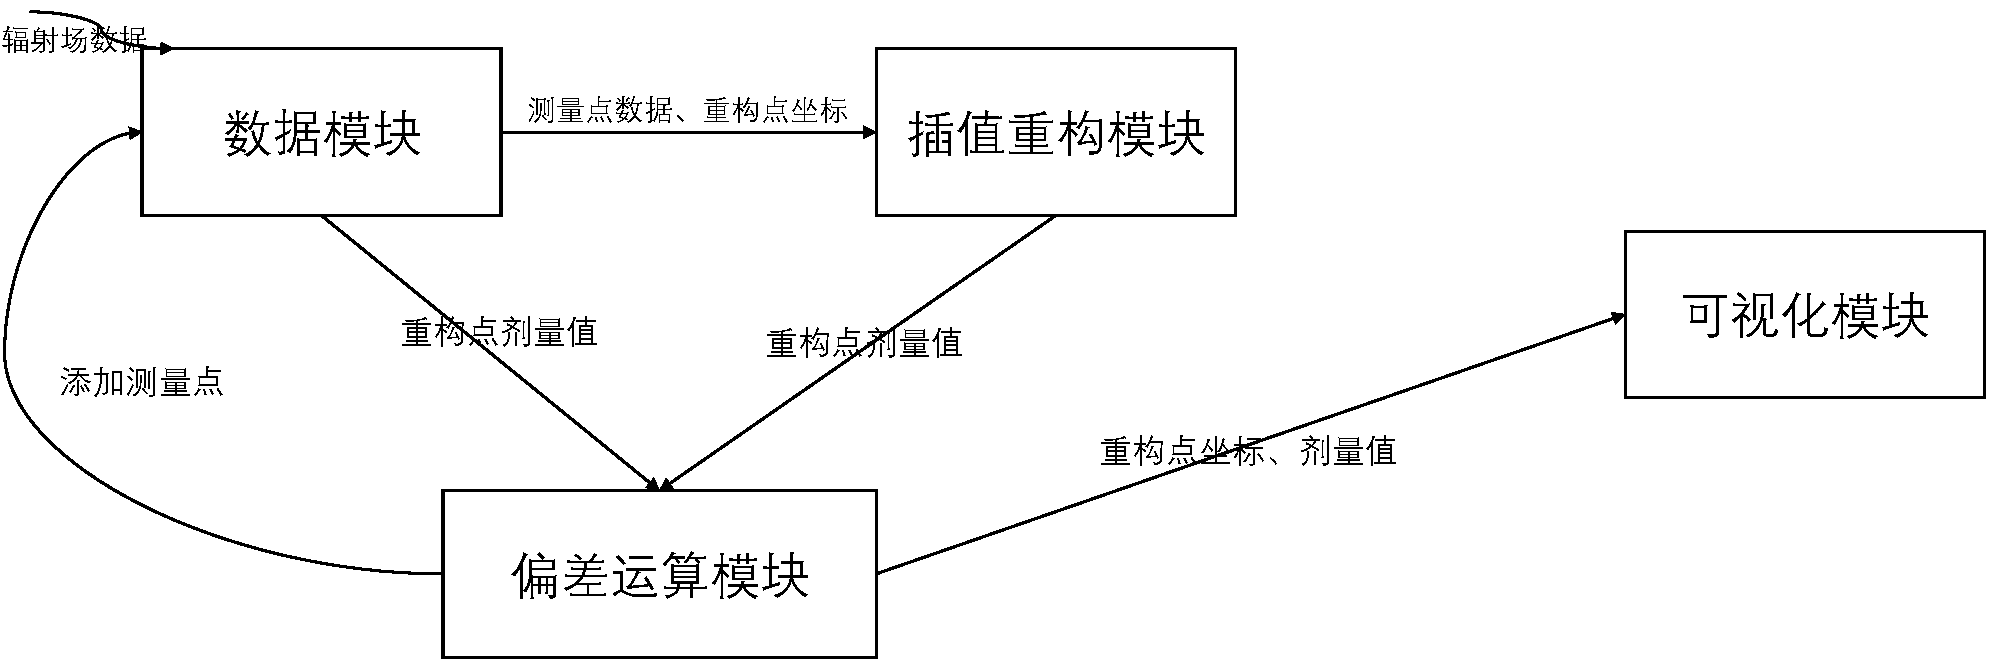
\includegraphics[width=1.0\textwidth]{figure/辐射场重构程序模块.pdf}
      \caption{空间辐射场三维重构方法程序模块化设计}
      \label{空间辐射场三维重构方法程序模块化设计}
\end{figure}
\begin{enumerate}
      \item 数据模块
            \newline 数据模块对辐射场整体数据进行处理以及对重构后偏差较大的点进行判断,该模块具体功能包括:
            \begin{itemize}
                  \item 处理Geant4输出数据,将数据按照csv格式进行存储;
                  \item 添加测量点数据,对于插值偏差较大的区域添加测量点,将其存储于测量点数据文件;
                  \item 整合重构点数据,将重构后的数据进行整理,存储为ROOT绘制所需文件类型;
            \end{itemize}
      \item 插值重构模块
            \newline 插值重构模块是空间辐射场三维重构程序中的核心模块,其中包含了两种插值算法——样条插值算法和克里金插值算法,其功能是通过两种重构算法对辐射场数据进行插值重构,得到插值重构场,并按权重对两种辐射场数据进行组合,最终得到合适的辐射场;
      \item 偏差运算模块
            \newline 偏差运算模块为辐射场三维重构程序的重要模块,该模块为本论文提出的插值重构方法中最关键的创新点实现的模块。该模块实现的功能为计算重构辐射场与Geant4模拟辐射场中各个坐标点的偏差,对于样条插值重构辐射场与克里金插值重构辐射场偏差较大的区域,选择一个点作为测量点;
      \item 可视化模块
            \newline 可视化模块是基于计算机的图像处理技术,将辐射场插值重构数据以更直观的形式展现出来,从而使得重构辐射场能够在ALARA设计分析、辐射剂量估算等领域得到更好的应用。
\end{enumerate}

数据模块先从Geant4模拟中得到辐射场数据,通过数据处理,转换为与插值重构算法模块能够耦合的数据类型,然后存储为csv格式;插值重构模块将处理后的数据进行读取、插值重构,分别将样条插值法和克里金插值法重构的辐射场数据进行输出;偏差运算模块得到两个辐射场重构数据后,将其进行偏差计算,若偏差值大于设定偏差量,则将插值区域输出至数据模块,让其进行再次测量,直至两种算法重构的辐射场偏差值在设定范围内,将其辐射场数值进行输出;可视化模块根据重构辐射场数据,将辐射场进行图像绘制。

在辐射场重构方法程序各模块设计基础上,考虑其实现的方法论及相应算法,总程序采用高内聚、低耦合的设计思想,尽可能将内容内聚、数据耦合,形成模块内功能内部连续,外部通过数据接口进行连接。本论文采用的辐射场重构算法的程序框图如图\ref{辐射场重构算法程序框图}所示。

\begin{figure}
      \centering
      \begin{tikzpicture}[node distance=10pt]
            \node[draw, rounded corners]                        (start)   {开始};
            \node[draw, below=of start]                         (step 1)  {导入数据};
            \node[draw, below=of step 1]                        (step 2)  {计算Kriging插值重构辐射场};
            \node[draw, below=of step 2]                        (step 3)  {计算Spline插值重构辐射场};
            \node[draw, below=of step 3]                        (step 4)  {计算两个重构辐射场的偏差};
            \node[draw, diamond, aspect=6, below=of step 4]     (choice)  {偏差值是否大于设定值};
            \node[draw, right=20pt of choice]                   (step x)  {添加测量数据};
            \node[draw, below=20pt of choice]                   (step 5)  {绘制空间辐射场};
            \node[draw, below=of step 5]                        (step 6)  {计算整体偏差};
            \node[draw, rounded corners, below=of step 6]       (end)     {结束};

            \draw[->] (start)  -- (step 1);
            \draw[->] (step 1) -- (step 2);
            \draw[->] (step 2) -- (step 3);
            \draw[->] (step 3) -- (step 4);
            \draw[->] (step 4) -- (choice);
            \draw[->] (choice) -- (step 5);
            \draw[->] (choice) -- node[left]  {否} (step 5);
            \draw[->] (choice) -- node[above] {是}  (step x);
            \draw[->] (step 5) -- (step 6);
            \draw[->] (step x) -- (step x|-step 1) -> (step 1);
            \draw[->] (step 6) -- (end);
      \end{tikzpicture}
      \caption{辐射场重构算法程序框图}
      \label{辐射场重构算法程序框图}
\end{figure}

下面介绍该程序每一步骤所实现的方式:
\begin{enumerate}
      \renewcommand{\labelenumi}{(\theenumi)}
      \item 导入数据:
            \newline 辐射场可视化数据包括测量点数据文件、插值点坐标数据文件以及插值点辐射场剂量数据文件,导入数据步骤将三个文件分别按照各文件存储格式进行导入指定目录下;
      \item 计算Kriging插值重构辐射场:
            \newline Kriging插值算法采用普通克里金模型,变异函数采用指数函数,具体计算方法原理及算法见第三章。本论文Kriging插值算法基于日本GIS公司开发的开源框架Polatory开发,Polatory框架是基于径向基函数(RBF)插值的快速、高效框架;
      \item 计算Spline插值重构辐射场:
            \newline Spline插值算法具体原理以及算法见第二章,本论文采用的样条插值算法为多层B样条插值算法(MBA),本论文的辐射场样条插值算法是基于俄罗斯科学院研究员Denis Demidov在Github开源平台开源的mba库,mba库是基于Seungyong Lee发表的《使用多层B样条进行散乱数据插值》论文中多层B样条插值算法\textsuperscript{\cite{Lee1997}}编写;
      \item 计算两个重构辐射场的偏差:
            \newline 通过Kriging插值和Spine插值后,得到两个不同的辐射场数据,通过计算两个辐射场的相对偏差(relative deviation),来决定是否需要添加测量点来优化辐射场重构效果。相对偏差计算公式如下:
            \begin{equation}
                  RD = \frac{| v_{k} - v_{s} |}{\frac{1}{2}(v_{k} + v_{s})} \times 100\%
                  \label{辐射场偏差公式}
            \end{equation}
            其中RD表示辐射场相对偏差;$ v_{k} $代表克里金插值算法重构出的插值;$ v_{s} $代表多层B样条插值算法重构出的插值;
      \item 判断偏差值是否大于设定值:
            \newline 通过上一步骤计算得到整个辐射场两种重构方法重构的偏差值之后,对其偏差较大的区域(大于设定偏差值),选取该区域内最大的偏差点进行再次测量;
      \item 添加测量数据:
            \newline 将上一步骤中得到的偏差最大的点的数据添加到测量点数据文件中,保存为相应格式;
      \item 绘制空间辐射场:
            \newline 获得到重构辐射场数据后,将数据保存为root格式,使用ROOT进行绘制,具体步骤在下一节中进行详细介绍;
      \item 计算整体偏差:
            \newline 在获得重构辐射场数据后,将辐射场插值数据与模拟数据进行计算,比较辐射场重构方法的重构效果。
\end{enumerate}